Esta librería es la encargada de modelar un documento NCL. Contiene clases para representar cada sección de dicho documento, tal como regiones, descriptores, medias, transiciones, etc.
Los objetos de esta librería prácticamente no tienen comportamiento, ya que su único propósito es el de modelado de datos.
La clase principal es \texttt{NclDocument}, que como su nombre lo indica representa al documento NCL. A partir de la instancia de dicha clase se referencian los objetos que representan cada sección del NCL, armando así el modelo.
Cada objeto guarda información sobre las propiedades que le fueron seteadas desde el archivo NCL. Por ejemplo \texttt{LayoutRegion} tiene información sobre las dimensiones de la región.
\emph{ncl30-converter} es el encargado de instanciar las clases de \emph{ncl30} a medida que realiza el parsing.
	
\begin{figure}[h!]
	\centering
	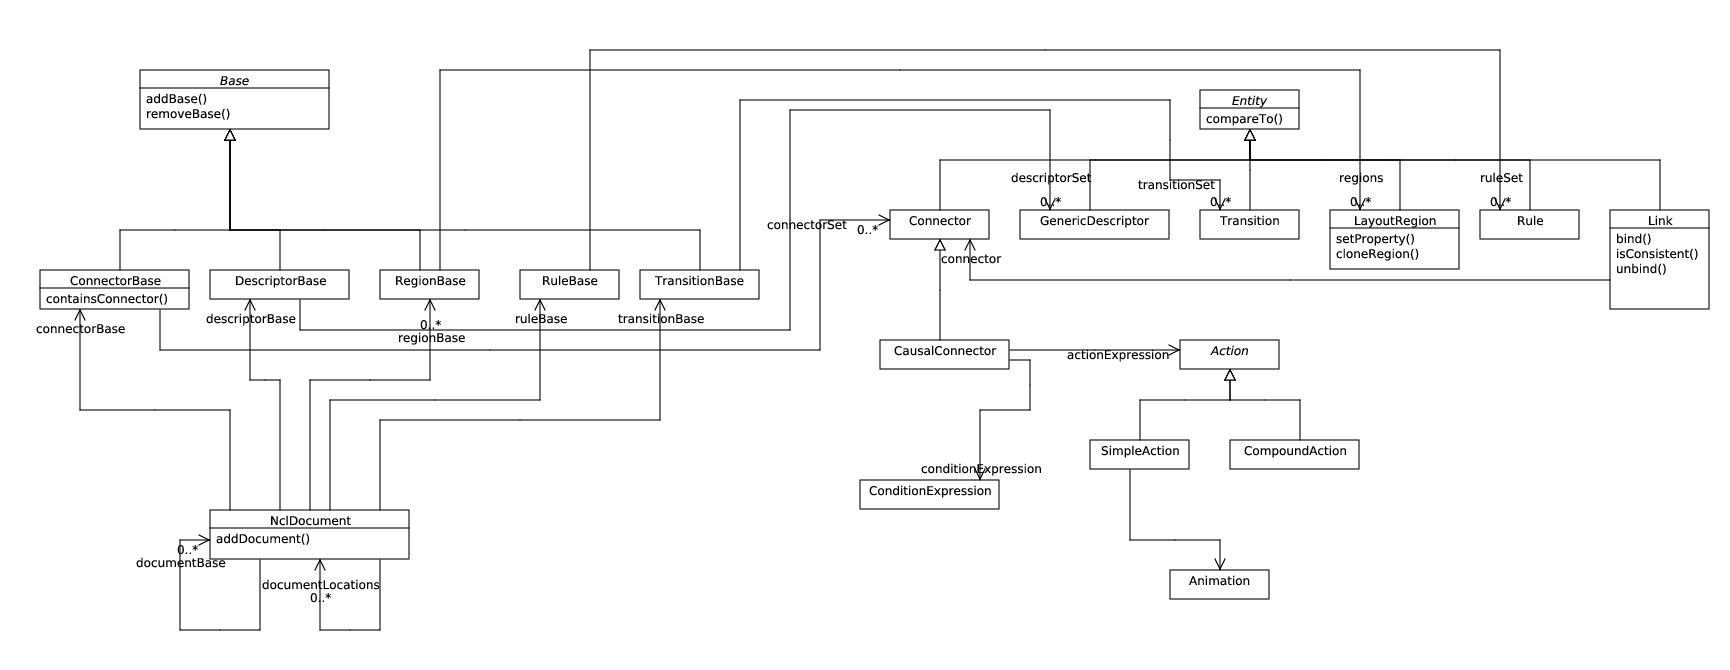
\includegraphics[scale=0.26]{resources/uml-ncl30.jpg}
	\caption{Diagrama de las principales clases de la librería \emph{ncl30}.}
\end{figure}

\FloatBarrier
